%%%%%%%%%%%%%%%%%%%%%%%%%%%%%%%%%%%%%%%%%
% Stylish Article
% LaTeX Template
% Version 2.1 (1/10/15)
%
% This template has been downloaded from:
% http://www.LaTeXTemplates.com
%
% Original author:
% Mathias Legrand (legrand.mathias@gmail.com) 
% With extensive modifications by:
% Vel (vel@latextemplates.com)
%
% License:
% CC BY-NC-SA 3.0 (http://creativecommons.org/licenses/by-nc-sa/3.0/)
%
%%%%%%%%%%%%%%%%%%%%%%%%%%%%%%%%%%%%%%%%%

%----------------------------------------------------------------------------------------
%	PACKAGES AND OTHER DOCUMENT CONFIGURATIONS
\usepackage{placeins}
\usepackage{float}
%----------------------------------------------------------------------------------------

\documentclass[fleqn,10pt]{SelfArx} % Document font size and equations flushed left

\usepackage[english]{babel} % Specify a different language here - english by default

\usepackage{lipsum} % Required to insert dummy text. To be removed otherwise

%----------------------------------------------------------------------------------------
%	COLUMNS
%----------------------------------------------------------------------------------------

\setlength{\columnsep}{0.55cm} % Distance between the two columns of text
\setlength{\fboxrule}{0.75pt} % Width of the border around the abstract

%----------------------------------------------------------------------------------------
%	COLORS
%----------------------------------------------------------------------------------------

\definecolor{color1}{RGB}{0,0,90} % Color of the article title and sections
\definecolor{color2}{RGB}{0,20,20} % Color of the boxes behind the abstract and headings

%----------------------------------------------------------------------------------------
%	HYPERLINKS
%----------------------------------------------------------------------------------------

\usepackage{hyperref} % Required for hyperlinks
\hypersetup{hidelinks,colorlinks,breaklinks=true,urlcolor=color2,citecolor=color1,linkcolor=color1,bookmarksopen=false,pdftitle={Title},pdfauthor={Author}}

%----------------------------------------------------------------------------------------
%	ARTICLE INFORMATION
%----------------------------------------------------------------------------------------

\JournalInfo{Text Mining \& Search Project} % Journal information
\Archive{A.Y. 2019-2020} % Additional notes (e.g. copyright, DOI, review/research article)

\PaperTitle{Methodological approaches for Text Summarization} % Article title

\Authors{\textbf{Riccardo Cervero}, \textbf{794126}\textsuperscript{*}} % Authors
\affiliation{\textsuperscript{*}\textit{Universita` degli Studi di Milano Bicocca, CdLM in Data Science}} 

\Keywords{Abstractive Summarization --- Extractive Summarization} % Keywords - if you don't want any simply remove all the text between the curly brackets
\newcommand{\keywordname}{Keywords} % Defines the keywords heading name

%----------------------------------------------------------------------------------------
%	ABSTRACT
%----------------------------------------------------------------------------------------

\Abstract{}

%----------------------------------------------------------------------------------------

\begin{document}

\flushbottom % Makes all text pages the same height

\maketitle % Print the title and abstract box

\tableofcontents % Print the contents section

\thispagestyle{empty} % Removes page numbering from the first page

%----------------------------------------------------------------------------------------
%	ARTICLE CONTENTS
%----------------------------------------------------------------------------------------

\section{Dataset Exploration} 
The texts to be summarized hails from a portion of the \href{https://www.kaggle.com/snap/amazon-fine-food-reviews}{"Fine Food Reviews"} dataset, recording 100,000 natural-language-written reviews in English from more than 70,000 Amazon users. The original data span from October 1999 up to October 2012, including, besides plain text reviews, product and user information, ratings and, above all, a very brew reference summary offered by database providers which will constitute the ground truth during the neural network training phase and an evaluation benchmark.\\
As seen from the plot, ratings distribution is heavily unbalanced towards most positive score.
\par
{\centering\vspace{10pt}
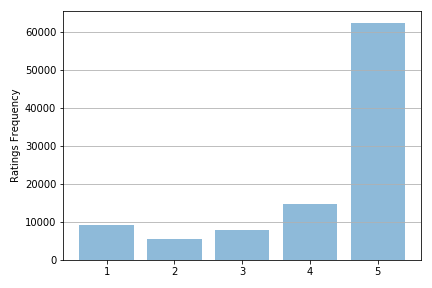
\includegraphics[width=8cm, height=5cm]{r_dist.png}
\captionof{figure}{Ratings distribution\label{fig:img1}}
\vspace{10pt}
\par}
As far as reviews, the average number of sentences is 5, while about one sentence on average is used to summarize the content. The number of sentences in the original document can affect extractive results of summarization, and its distribution shows, in the first case, a slight concentration around the mean\footnote{Reviews composed by a number of sentences between 3 and 7 are about 64\% of the total.}, with a very long and thin tail.\par
{\centering\vspace{10pt}
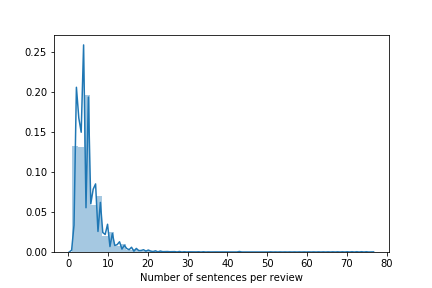
\includegraphics[width=9cm, height=5cm]{text_dist.png}
\captionof{figure}{Distribution of number of sentence per review\label{fig:img1}}
\vspace{10pt}
\par}
Nevertheless, even though this characteristic of homogeneity could help avoid bias during generation and comparison of several summaries, it is counterbalanced by a greater variability\footnote{While coefficient of variance for sentences count is about 74\%, the one related to word count is 102\%} in the number of words per review.
\par
{\centering\vspace{10pt}
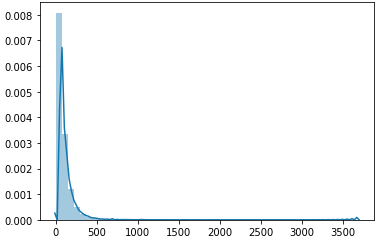
\includegraphics[width=8.2cm, height=4.2cm]{word_dist.png}
\captionof{figure}{Distribution of number of word per review\label{fig:img1}}
\vspace{10pt}
\par}
Finally, it is possible to get a first insight on vocabulary composition by representing the corpus \textit{wordcloud}. 
\par
{\centering\vspace{10pt}
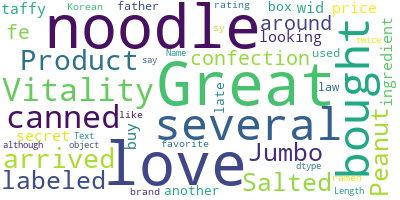
\includegraphics[width=8.2cm, height=4.2cm]{wc.png}
\captionof{figure}{Corpus WordCloud\label{fig:img1}}
\vspace{10pt}
\par}
%------------------------------------------------
\section{Text Pre-processing}
Review is a particular kind of text, often composed by neither non-professional writer nor journalist which thus tends to resemble spoken language, because includes abbreviations, slang and informal phrases, errors in punctuation and misspellings, etc. This documents appear as a mixture of heterogeneous forms of text, even presenting different lexical and syntactic structures within the same document. For this reason, pre-processing operations are compulsory to help reduce distortion and try to convert the corpus into standard form. This goal is achieved in a preliminary way through the following operations. After having tokenized\footnote{Separator character used is \textit{white-space}.} the document, as text normalization phase, it is necessary to convert all informal expressions that occur in form of contractions\footnote{Such as \textit{couldn't}, which should be replaced by \textit{could not}} and put all the tokens to lower case. The second step consist in removing noisy part of the text to be analyzed: genitives, punctuation, symbols, special characters and numbers. Finally, stop words are eliminated because this very frequent tokens are useless and could distort the co-occurrence analysis during the stage of text representation. Neither stemming nor lematization operations are performed, because inflected and derived tokens provide fundamental information that both simplest algorithms and neural network cannot afford to lose during elaboration of a summary containing the most relevant concepts.\\
In each following methodology, the aforementioned operations will be applied separately to each sentence extracted from the text by means of a \textit{sentence tokenizer}, so as to return a list of \textit{cleaned} sentences. The \textit{sentence tokenizer} uses an unsupervised algorithm to build a model for detecting sentence boundaries\footnote{Algorithm is called \href{https://www.nltk.org/_modules/nltk/tokenize/punkt.html}{\texttt{PunktSentenceTokenizer}}.}, which has proven to be an effective approach for many European languages.
%------------------------------------------------
\section{Extractive Summarization}
Extractive summarization aims to recognize most important sections of a text to generate a subset of the sentences. Between the two approaches, this is certainly the most superficial, as it returns a simple verbatim reduction of the original document.
\subsection{Topic representation methods}
These methods generate an intermediate representation capturing discussed topics and score each sentence according to its importance. This class includes methods that vary mainly on the basis of the intermediate representation that they are able to extract. One of them is the matrix factorization based Latent Semantic Analysis.
\subsubsection{Latent Semantic Analysis}
Latent Semantic Analysis (\textit{LSA}) is an unsupervised technique extracting an implicit representation of semantics within text identifies several. It identifies several patterns of co-occurring words as weighted relevant topics, without using lexical resources. Based on distributional hypothesis, assumes that words close in meaning will occur in similar location of text, thus, in case of text summarization, in same sentences. In this way, it is possible to understand which sentence deals with which topic and to select sentences related to most important themes.
The algorithm is implemented with following steps. Topics representation starts with filling an $nxm$ matrix $A$, each row corresponding to an input word and each column to a sentence. Each entry $a_{ij}$ records the weight of the i-th word in the j-th sentence, zero if the word is not contained in the sentence. Non-zero values can be of three types:
\begin{itemize}
  \item Term Frequency $tf_{t,s}$, which is not convenient because does not consider the different number of words within a sentence. In fact, it is better that weights of words from a short sentence are bigger, as we can say they exerts more influence;
  \item Term Frequency normalized by sentence length $\frac{tf_{t,s}}{|s|}$
  \item Tf-idf $$tf.idf=\frac{tf_{t,s}}{|s|}\bullet log(\frac{N}{df_t})$$ which derives from the product between $tf$ and \textit{inverse document frequency} $idf$. This value proportionally measures both frequency in the single sentence and the diffusion in the other ones, thus increasing with the rarity of the term in the collection, that is the specificity of that term in relation to that sentence. For this reason, it is the most correct weighting function for this type of co-occurence analysis.  
\end{itemize}
Matrix $A$ can be decomposed into three sub-matrices:
$$A=U\Sigma V^T$$
where:
\begin{itemize}
    \item $U$ records the weight of each word for each topic
    \item $\Sigma$ is a diagonal matrix whose non-zero values represent topic importance
    \item $V^T$ consists of a new representation of the sentences, each expressed no longer in terms of the words it contains but in terms of the topics it relates to:
\end{itemize}
The product $D=\Sigma V^T$ combines topic importance scores with the new representation of the sentences and indicates to what extent the sentence communicates a certain topic. Therefore, $d_{ij}$ is the weight of the argument i for the sentence j.\\
Sentences presenting many of the most important topics - based on weights recorded in $\Sigma$ matrix - are often excellent candidates for the summary. For this reason, the algorithm identifies these candidates by calculating for each sentence  $$s_i=\sqrt{\sum_{j=1}^md^2_{ij}}$$
\\
As anticipated, when the algorithm uses the term frequency divided by the length, it tends to favor shorter sentences with frequent terms, while exploiting tf.idf function it operates an additional filter on those sentences that contain rarer words, those more "specialized" with respect to the topic. On the contrary, application of simple term frequency weights only makes method focus on the raw number of times a word occurs.
\subsection{Indicator Representation methods}
Original text can also be analyzed by means of a set of relevance indicators, which do not aim to discover topics. In this case, each sentence is indeed described by a list of features - such as length of the sentence, position in the document, presence of certain words, etc -, which can be then combined - within a graph or using Machine Learning techniques -, to obtain a unique scoring useful to rank and select most important sentences. Three different approaches have been implemented.
\subsubsection{Graph-based: TextRank}
Graph-based summarization methodologies derive from PageRank algorithm, which assigns numerical weights to the related elements of a set, with the aim of quantifying the relative importance within the group. In this case, the method will represent the entire review as a network of inter-connected sentences, each one associated with a node. Edges join these vertices if and only if the similarity between the two given sentences exceeds a certain threshold. At the end, graph representation will return two outputs:
\begin{itemize}
    \item the graph partition from which it is possible to deduce a set of discrete topics extracted from the corpus 
    \item important sentences, namely those connected with many of the others in the partition, and which will most likely be included in the summary
\end{itemize}
Among all the existing variants, the most popular was chosen: the \textit{TextRank} algorithm. First of all, \textit{TextRank} splits the review into sentences - with the aforementioned \textit{sentence tokenizer} - and applies pre-processing operations to them.\\
Then, a vector representation for every sentence has to be produced. An alternative would be to resort to the weighting functions used with \textit{LSA}, but using them to measure similarity would bring a strong limitation, because they do not take into account syntactic and semantic information, like the order of the words. For this reason, sentences will be represented through the word embeddings produced by the pre-trained model called \textit{"Global Vectors for Word Representation"} \textit{GloVe}. GloVe is an unsupervised learning algorithm for obtaining words vector representations\footnote{Precisely, we will be using the pre-trained \textit{Wikipedia 2014 + Gigaword 5 GloVe} vectors}. This embeddings are created by mapping words into a space where the distances are related to semantic similarity. Training is performed by extracting global statistical information from the non-zero values of a co-occurence word-word matrix, rather than 
from the entire sparse matrix - like matrix factorization methods do - or from the single context window within the large corpus, - like \textit{word2vec} does. The resulting representations show interesting linear substructures of the word vector space.\\
\textit{GloVe} will thus consider 400k terms\footnote{If otherwise embedding of one word does not exist, the algorithm returns a vector of zeros.}, each one described by an array of 100 values. Finally, sentences vector representation will be obtained by computing the mean of all the vectors representing each word in the given sentence, gaining a consolidated vector for the sentence.\\
The third step consists in compute the cosine similarity among all the sentence vectors and store it into a $nxn$ matrix.\\
This similarity matrix is converted into a graph, with sentences as vertices and similarity scores as edges.\\
Hereafter, \textit{TextRank} implements \textit{PageRank} algorithm to extract an importance score, as aforementioned, and rank sentences based on their score. Finally, the final summary is created by selecting the top N sentences.
\subsubsection{TextRank variant}
This project also calls for the implementation of a packaged TextRank variant: \texttt{PytextRank}. This performs a lemmatization of the text, constructing a \textit{lemma graph} to represent links among the candidate sentences.
\subsubsection{Feature-based: Luhn's Algorithm}
Luhn's Algorithm is an early heuristic method which performs extractive summarization task by computing the “significance” of the word from the frequency. The significance in the document is interpreted as an evaluation of the relevance of a term within the sentence. The algorithm is a naive approach based on Tf-Idf representation and looking at the “window size” of non-important words among relevant words.\\
The stages are:
\begin{enumerate}
  \item Calculate signficant words in the text by means of a min and maximum ratio of occurence, ignoring most frequent words and least frequent ones 
  \item For each sentence in the text calculate its weight based on the number of keywords squared divided by the windows size, which is the maximum distance between two significant words
  \item Sort sentences in descending order based on their weight and output the first n of them.
\end{enumerate}


1. In the first stage, we try to determine which words are more significant towards the meaning of document. Luhn states that this is first done by doing a frequency analysis, then finding words which are significant, but not unimportant English words.
2. In the second phase, we find out the most common words in the document, and then take a subset of those that are not these most common english words, but are still important. It usually consists of following three steps:

It begins with transforming the content of sentences into a mathematical expression, or vector(represented below through binary representation). Here we use a bag of words , which ignores all the filler words. Filler words are usually the supporting words that do not have any impact on our document meaning. Then we count all the valuable words left to us. For example,
Mytable

In the above table we can clearly see that the words like an and a that are the stopwords are not considered while evaluation.

In this step we use evaluate sentences using sentence scoring technique. We can use the scoring method as illustrated below.
Score= (Number of meaningful words)2/(Span of meaningful words)
A span here refers to the part of sentence(in our case)/document consisting all the meaningful words.

Tf-idf can also be used in order to prioritize the words in a sentence.
Once the sentence scoring is complete, the last step is simply to select those sentences with the highest overall rankings.
\subsubsection{Deep Learning based: BERT Summarizer}
%------------------------------------------------
\section{Abstractive Summarization}
%------------------------------------------------
\section{Evaluation}
Only one sentence
%------------------------------------------------
\section{Results and Discussion}
%----------------------------------------------------------------------------------------
%	Code
%----------------------------------------------------------------------------------------
\section*{Code}
\href{https://github.com/RCrvro/Text-Summarization-Project}{Code is available at this link.}
%----------------------------------------------------------------------------------------
%	REFERENCE LIST

%----------------------------------------------------------------------------------------
\phantomsection
\bibliographystyle{unsrt}
\bibliography{sample}
GloVe: https://nlp.stanford.edu/projects/glove/

PyTextRank: https://pypi.org/project/pytextrank/

Luhn: http://courses.ischool.berkeley.edu/i256/f06/papers/luhn58.pdf

Edmundson: https://iq.opengenus.org/edmundson-heuristic-method-for-text-summarization/
%----------------------------------------------------------------------------------------

\end{document}
